%% abtex2-modelo-trabalho-academico.tex, v-1.9.6 laurocesar
%% Copyright 2012-2016 by abnTeX2 group at http://www.abntex.net.br/ 
%%
%% This work may be distributed and/or modified under the
%% conditions of the LaTeX Project Public License, either version 1.3
%% of this license or (at your option) any later version.
%% The latest version of this license is in
%%   http://www.latex-project.org/lppl.txt
%% and version 1.3 or later is part of all distributions of LaTeX
%% version 2005/12/01 or later.
%%
%% This work has the LPPL maintenance status `maintained'.
%% 
%% The Current Maintainer of this work is the abnTeX2 team, led
%% by Lauro César Araujo. Further information are available on 
%% http://www.abntex.net.br/
%%
%% This work consists of the files abntex2-modelo-trabalho-academico.tex,
%% abntex2-modelo-include-comandos and abntex2-modelo-references.bib
%%

% ------------------------------------------------------------------------
% ------------------------------------------------------------------------
% abnTeX2: Modelo de Trabalho Academico (tese de doutorado, dissertacao de
% mestrado e trabalhos monograficos em geral) em conformidade com 
% ABNT NBR 14724:2011: Informacao e documentacao - Trabalhos academicos -
% Apresentacao
% ------------------------------------------------------------------------
% ------------------------------------------------------------------------

\documentclass[
	% -- opções da classe memoir --
	12pt,				% tamanho da fonte
	openright,			% capítulos começam em pág ímpar (insere página vazia caso preciso)
	twoside,			% para impressão em recto e verso. Oposto a oneside
	a4paper,			% tamanho do papel. 
	% -- opções da classe abntex2 --
	%chapter=TITLE,		% títulos de capítulos convertidos em letras maiúsculas
	%section=TITLE,		% títulos de seções convertidos em letras maiúsculas
	%subsection=TITLE,	% títulos de subseções convertidos em letras maiúsculas
	%subsubsection=TITLE,% títulos de subsubseções convertidos em letras maiúsculas
	% -- opções do pacote babel --
	english,			% idioma adicional para hifenização
	french,				% idioma adicional para hifenização
	spanish,			% idioma adicional para hifenização
	brazil				% o último idioma é o principal do documento
	]{abntex2}

% ---
% Pacotes básicos 
% ---
\usepackage{lmodern}			% Usa a fonte Latin Modern			
\usepackage[T1]{fontenc}		% Selecao de codigos de fonte.
\usepackage[utf8]{inputenc}		% Codificacao do documento (conversão automática dos acentos)
\usepackage{lastpage}			% Usado pela Ficha catalográfica
\usepackage{indentfirst}		% Indenta o primeiro parágrafo de cada seção.
\usepackage{color}				% Controle das cores
\usepackage{graphicx}			% Inclusão de gráficos
\usepackage{microtype} 			% para melhorias de justificação
% ---
		
% ---
% Pacotes adicionais, usados apenas no âmbito do Modelo Canônico do abnteX2
% ---
\usepackage{lipsum}				% para geração de dummy text
% ---

% ---
% Pacotes de citações
% ---
\usepackage[brazilian,hyperpageref]{backref}	 % Paginas com as citações na bibl
\usepackage[alf]{abntex2cite}	% Citações padrão ABNT

% --- 
% CONFIGURAÇÕES DE PACOTES
% --- 

% ---
% Configurações do pacote backref
% Usado sem a opção hyperpageref de backref
\renewcommand{\backrefpagesname}{Citado na(s) página(s):~}
% Texto padrão antes do número das páginas
\renewcommand{\backref}{}
% Define os textos da citação
\renewcommand*{\backrefalt}[4]{
	\ifcase #1 %
		Nenhuma citação no texto.%
	\or
		Citado na página #2.%
	\else
		Citado #1 vezes nas páginas #2.%
	\fi}%
% ---

% ---
% Informações de dados para CAPA e FOLHA DE ROSTO
% ---
\titulo{Modelo Canônico de\\ Trabalho Acadêmico com \abnTeX}
\autor{Equipe \abnTeX}
\local{Brasil}
\data{2015, v-1.9.6}
\orientador{Lauro César Araujo}
\coorientador{Equipe \abnTeX}
\instituicao{%
  Universidade do Brasil -- UBr
  \par
  Faculdade de Arquitetura da Informação
  \par
  Programa de Pós-Graduação}
\tipotrabalho{Tese (Doutorado)}
% O preambulo deve conter o tipo do trabalho, o objetivo, 
% o nome da instituição e a área de concentração 
\preambulo{Modelo canônico de trabalho monográfico acadêmico em conformidade com
as normas ABNT apresentado à comunidade de usuários \LaTeX.}
% ---


% ---
% Configurações de aparência do PDF final

% alterando o aspecto da cor azul
\definecolor{blue}{RGB}{41,5,195}

% informações do PDF
\makeatletter
\hypersetup{
     	%pagebackref=true,
		pdftitle={\@title}, 
		pdfauthor={\@author},
    	pdfsubject={\imprimirpreambulo},
	    pdfcreator={LaTeX with abnTeX2},
		pdfkeywords={abnt}{latex}{abntex}{abntex2}{trabalho acadêmico}, 
		colorlinks=true,       		% false: boxed links; true: colored links
    	linkcolor=blue,          	% color of internal links
    	citecolor=blue,        		% color of links to bibliography
    	filecolor=magenta,      		% color of file links
		urlcolor=blue,
		bookmarksdepth=4
}
\makeatother
% --- 

% --- 
% Espaçamentos entre linhas e parágrafos 
% --- 

% O tamanho do parágrafo é dado por:
\setlength{\parindent}{1.3cm}

% Controle do espaçamento entre um parágrafo e outro:
\setlength{\parskip}{0.2cm}  % tente também \onelineskip

% ---
% compila o indice
% ---
\makeindex
% ---

\usepackage{amsthm,amsfonts}
\usepackage{amsmath}


%% Todos esses comandos devem sermigrados para outro arquivo em versões futuras
\newcommand{\setN}{\mathbb{N}}
\newcommand{\setE}{\mathbb{E}}
\newcommand{\setS}{\mathbb{S}}
\newcommand{\setT}{\mathbb{T}}

\newcommand{\setdp}{\delta_{+}}
\newcommand{\setdn}{\delta_{-}}
\newcommand{\edge}{\mathrm{e}}
\newcommand{\inode}{\mathrm{i}}
\newcommand{\jnode}{\mathrm{j}}
\newcommand{\dmin}{\mathrm{d_{min}}}
\newcommand{\dmax}{\mathrm{d_{max}}}
\newcommand{\phmin}{\mathrm{ph_{min}}}
\newcommand{\phmax}{\mathrm{ph_{max}}}
\newcommand{\dem}{\mathrm{dem}}
\newcommand{\DT}{\mathfrak{D}}
\newcommand{\z}{\mathrm{z}}
\newcommand{\C}{\mathrm{C}}
\newcommand{\q}{\mathrm{q}}
\newcommand{\tT}{\mathrm{t}}

\newcommand{\vQ}{\mathrm{Q}}
\newcommand{\vQF}{\mathrm{QF}}
\newcommand{\vQT}{\mathrm{QT}}
\newcommand{\vH}{\mathrm{H}}
\newcommand{\vD}{\mathrm{D}}





% ----
% Início do documento
% ----
\begin{document}

% Seleciona o idioma do documento (conforme pacotes do babel)
%\selectlanguage{english}
\selectlanguage{brazil}

% Retira espaço extra obsoleto entre as frases.
\frenchspacing 

% ----------------------------------------------------------
% ELEMENTOS PRÉ-TEXTUAIS
% ----------------------------------------------------------
% \pretextual

% ---
% Capa
% ---
\imprimircapa


% ---


% ---
% Folha de rosto
% (o * indica que haverá a ficha bibliográfica)
% ---
\imprimirfolhaderosto*
% ---

% ---
% Inserir a ficha bibliografica
% ---

% Isto é um exemplo de Ficha Catalográfica, ou ``Dados internacionais de
% catalogação-na-publicação''. Você pode utilizar este modelo como referência. 
% Porém, provavelmente a biblioteca da sua universidade lhe fornecerá um PDF
% com a ficha catalográfica definitiva após a defesa do trabalho. Quando estiver
% com o documento, salve-o como PDF no diretório do seu projeto e substitua todo
% o conteúdo de implementação deste arquivo pelo comando abaixo:
%
% \begin{fichacatalografica}
%     \includepdf{fig_ficha_catalografica.pdf}
% \end{fichacatalografica}

%%\begin{fichacatalografica}
%%	\sffamily
%%	\vspace*{\fill}					% Posição vertical
%%	\begin{center}					% Minipage Centralizado
%%	\fbox{\begin{minipage}[c][8cm]{13.5cm}		% Largura
%%	\small
%%	\imprimirautor
%%	%Sobrenome, Nome do autor
%%	
%%	\hspace{0.5cm} \imprimirtitulo  / \imprimirautor. --
%%	\imprimirlocal, \imprimirdata-
%%	
%%	\hspace{0.5cm} \pageref{LastPage} p. : il. (algumas color.) ; 30 cm.\\
%%	
%%	\hspace{0.5cm} \imprimirorientadorRotulo~\imprimirorientador\\
%%	
%%	\hspace{0.5cm}
%%	\parbox[t]{\textwidth}{\imprimirtipotrabalho~--~\imprimirinstituicao,
%%	\imprimirdata.}\\
%%	
%%	\hspace{0.5cm}
%%		1. Palavra-chave1.
%%		2. Palavra-chave2.
%%		2. Palavra-chave3.
%%		I. Orientador.
%%		II. Universidade xxx.
%%		III. Faculdade de xxx.
%%		IV. Título 			
%%	\end{minipage}}
%%	\end{center}
%%\end{fichacatalografica}
% ---

% ---
% Inserir errata
% ---
%%\begin{errata}
%%Elemento opcional da \citeonline[4.2.1.2]{NBR14724:2011}. Exemplo:
%%
%%\vspace{\onelineskip}
%%
%%FERRIGNO, C. R. A. \textbf{Tratamento de neoplasias ósseas apendiculares com
%%reimplantação de enxerto ósseo autólogo autoclavado associado ao plasma
%%rico em plaquetas}: estudo crítico na cirurgia de preservação de membro em
%%cães. 2011. 128 f. Tese (Livre-Docência) - Faculdade de Medicina Veterinária e
%%Zootecnia, Universidade de São Paulo, São Paulo, 2011.
%%
%%\begin{table}[htb]
%%\center
%%\footnotesize
%%\begin{tabular}{|p{1.4cm}|p{1cm}|p{3cm}|p{3cm}|}
%%  \hline
%%   \textbf{Folha} & \textbf{Linha}  & \textbf{Onde se lê}  & \textbf{Leia-se}  \\
%%    \hline
%%    1 & 10 & auto-conclavo & autoconclavo\\
%%   \hline
%%\end{tabular}
%%\end{table}
%%
%%\end{errata}
% ---

% ---
% Inserir folha de aprovação
% ---

% Isto é um exemplo de Folha de aprovação, elemento obrigatório da NBR
% 14724/2011 (seção 4.2.1.3). Você pode utilizar este modelo até a aprovação
% do trabalho. Após isso, substitua todo o conteúdo deste arquivo por uma
% imagem da página assinada pela banca com o comando abaixo:
%
% \includepdf{folhadeaprovacao_final.pdf}
%
%%\begin{folhadeaprovacao}
%%
%%  \begin{center}
%%    {\ABNTEXchapterfont\large\imprimirautor}
%%
%%    \vspace*{\fill}\vspace*{\fill}
%%    \begin{center}
%%      \ABNTEXchapterfont\bfseries\Large\imprimirtitulo
%%    \end{center}
%%    \vspace*{\fill}
%%    
%%    \hspace{.45\textwidth}
%%    \begin{minipage}{.5\textwidth}
%%        \imprimirpreambulo
%%    \end{minipage}%
%%    \vspace*{\fill}
%%   \end{center}
%%        
%%   Trabalho aprovado. \imprimirlocal, 24 de novembro de 2012:
%%
%%   \assinatura{\textbf{\imprimirorientador} \\ Orientador} 
%%   \assinatura{\textbf{Professor} \\ Convidado 1}
%%   \assinatura{\textbf{Professor} \\ Convidado 2}
%%   %\assinatura{\textbf{Professor} \\ Convidado 3}
%%   %\assinatura{\textbf{Professor} \\ Convidado 4}
%%      
%%   \begin{center}
%%    \vspace*{0.5cm}
%%    {\large\imprimirlocal}
%%    \par
%%    {\large\imprimirdata}
%%    \vspace*{1cm}
%%  \end{center}
%%  
%%\end{folhadeaprovacao}
% ---

% ---
% Dedicatória
% ---
%%\begin{dedicatoria}
%%   \vspace*{\fill}
%%   \centering
%%   \noindent
%%   \textit{ Este trabalho é dedicado às crianças adultas que,\\
%%   quando pequenas, sonharam em se tornar cientistas.} \vspace*{\fill}
%%\end{dedicatoria}
% ---

% ---
% Agradecimentos
% ---
%%\begin{agradecimentos}
%%Os agradecimentos principais são direcionados à Gerald Weber, Miguel Frasson,
%%Leslie H. Watter, Bruno Parente Lima, Flávio de Vasconcellos Corrêa, Otavio Real
%%Salvador, Renato Machnievscz\footnote{Os nomes dos integrantes do primeiro
%%projeto abn\TeX\ foram extraídos de
%%\url{http://codigolivre.org.br/projects/abntex/}} e todos aqueles que
%%contribuíram para que a produção de trabalhos acadêmicos conforme
%%as normas ABNT com \LaTeX\ fosse possível.
%%
%%Agradecimentos especiais são direcionados ao Centro de Pesquisa em Arquitetura
%%da Informação\footnote{\url{http://www.cpai.unb.br/}} da Universidade de
%%Brasília (CPAI), ao grupo de usuários
%%\emph{latex-br}\footnote{\url{http://groups.google.com/group/latex-br}} e aos
%%novos voluntários do grupo
%%\emph{\abnTeX}\footnote{\url{http://groups.google.com/group/abntex2} e
%%\url{http://www.abntex.net.br/}}~que contribuíram e que ainda
%%contribuirão para a evolução do \abnTeX.
%%
%%\end{agradecimentos}
% ---

% ---
% Epígrafe
% ---
%%\begin{epigrafe}
%%    \vspace*{\fill}
%%	\begin{flushright}
%%		\textit{``Não vos amoldeis às estruturas deste mundo, \\
%%		mas transformai-vos pela renovação da mente, \\
%%		a fim de distinguir qual é a vontade de Deus: \\
%%		o que é bom, o que Lhe é agradável, o que é perfeito.\\
%%		(Bíblia Sagrada, Romanos 12, 2)}
%%	\end{flushright}
%%\end{epigrafe}
% ---

% ---
% RESUMOS
% ---

% resumo em português
%%\setlength{\absparsep}{18pt} % ajusta o espaçamento dos parágrafos do resumo
%%\begin{resumo}
%% Segundo a \citeonline[3.1-3.2]{NBR6028:2003}, o resumo deve ressaltar o
%% objetivo, o método, os resultados e as conclusões do documento. A ordem e a extensão
%% destes itens dependem do tipo de resumo (informativo ou indicativo) e do
%% tratamento que cada item recebe no documento original. O resumo deve ser
%% precedido da referência do documento, com exceção do resumo inserido no
%% próprio documento. (\ldots) As palavras-chave devem figurar logo abaixo do
%% resumo, antecedidas da expressão Palavras-chave:, separadas entre si por
%% ponto e finalizadas também por ponto.
%%
%% \textbf{Palavras-chave}: latex. abntex. editoração de texto.
%%\end{resumo}

% resumo em inglês
%%\begin{resumo}[Abstract]
%% \begin{otherlanguage*}{english}
%%   This is the english abstract.
%%
%%   \vspace{\onelineskip}
%% 
%%   \noindent 
%%   \textbf{Keywords}: latex. abntex. text editoration.
%% \end{otherlanguage*}
%%\end{resumo}

% resumo em francês 
%%\begin{resumo}[Résumé]
%% \begin{otherlanguage*}{french}
%%    Il s'agit d'un résumé en français.
%% 
%%   \textbf{Mots-clés}: latex. abntex. publication de textes.
%% \end{otherlanguage*}
%%\end{resumo}

% resumo em espanhol
%%\begin{resumo}[Resumen]
%% \begin{otherlanguage*}{spanish}
%%   Este es el resumen en español.
%%  
%%   \textbf{Palabras clave}: latex. abntex. publicación de textos.
%% \end{otherlanguage*}
%%\end{resumo}
% ---

% ---
% inserir lista de ilustrações
% ---
%%\pdfbookmark[0]{\listfigurename}{lof}
%%\listoffigures*
%%\cleardoublepage
% ---

% ---
% inserir lista de tabelas
% ---
%%\pdfbookmark[0]{\listtablename}{lot}
%%\listoftables*
%%\cleardoublepage
% ---

% ---
% inserir lista de abreviaturas e siglas
% ---
%%\begin{siglas}
%%  \item[ABNT] Associação Brasileira de Normas Técnicas
%%  \item[abnTeX] ABsurdas Normas para TeX
%%\end{siglas}
% ---

% ---
% inserir lista de símbolos
% ---
%%\begin{simbolos}
%%  \item[$ \Gamma $] Letra grega Gama
%%  \item[$ \Lambda $] Lambda
%%  \item[$ \zeta $] Letra grega minúscula zeta
%%  \item[$ \in $] Pertence
%%\end{simbolos}
% ---

% ---
% inserir o sumario
% ---
\pdfbookmark[0]{\contentsname}{toc}
\tableofcontents*
\cleardoublepage
% ---



% ----------------------------------------------------------
% ELEMENTOS TEXTUAIS
% ----------------------------------------------------------
\textual

% ----------------------------------------------------------
% Introdução (exemplo de capítulo sem numeração, mas presente no Sumário)
% ----------------------------------------------------------
\chapter*[Introdução]{Introdução}
\addcontentsline{toc}{chapter}{Introdução}
% ----------------------------------------------------------


A partir do momento em que o ser humano tornou-se sedentário surgiu a necessidade de que abastecimentos às pessoas fossem feitos, dentre muitos outros, destaca-se aqui o abastecimento de água.

A necessidade de utilização da água para abastecimento e indissociável da história da humanidade. Essa demanda determinou a própria localização das comunidades, desde que o homem passou a viver de forma sedentária, adotando a agricultura como meio de subsistência e abandonando a vida nômade, mais centrada na caça. A vida sedentária tornou mais complexo o equacionamento das demandas de água, que passaram então a
incluir o abastecimento de populações - e não mais de indivíduos ou famílias - tanto para atender as necessidades fisiológicas das pessoas, preparar alimentos e promover a limpeza, quanto para manter a agricultura, irrigando as culturas, \citeonline{heller2006}.

De acordo com \citeonline{rocha2009} o primeiro sistema de distribuição de água surgiu há cerca de 4.500 anos, mas a humanidade aprendeu a armazena-la para benefício próprio muito antes. Potes de barro não-cozidos foram fabricados por volta de 9000 a.C, e a cerâmica, em 7000 a.C., passando a ser fundamental para o incremento da capacidade de armazenamento de água. A irrigação começa a ser utilizada em 5000 a.C., na Mesopotâmia e no Egito,juntamente com os canais de drenagem, os quais recuperaram áreas pantanosas do delta do Nilo e dos rios Tigre e Eufrates. A primeira represa para armazenar água foi construída no Egito, em 2900 a.C., pelo faraó Menes, para abastecer a capital, Memphis, e a primeira represa de pedra foi erguida pelos assírios em 1300 a.C. O primeiro aqueduto conhecido foi criado em 700 a.C. por Ezequiel, rei de Judá, para abastecer jerusalém. Em 691 a.C., Senaqueribe, da Assíria, construiu um canal de 80 km e um aqueduto de 330 metros.

Há cerca de 4 mil anos foi construído pelos hindus o primeiro sistema eficiente de distribuição de água em Mohenjo-Daro, no vale do Indo, na Índia. Na época, Mohenjo-Daro devia ter cerca de 40 mil habitantes e um perfeito sistema de poços e canais de lançamentos de efluentes. Grandes obras de saneamento foram desenvolvidas já nas antigas Grécia e Roma com elevado padrão de engenharia civil e hidráulica. Os imensos aquedutos romanos, construídos para transporte de água das fontes situadas nas montanhas até as cidades, utilizando a gravidade, são atualmente visitados por centenas de turistas. A população abastecia-se de água em fontes e utilizava latrinas, ambas públicas, \cite{rocha2009}. 

Vários registros de experiências de suprimento de água são encontrados, desde a antiguidade, demonstrando o progressivo desenvolvimento de tecnologias para a captação, o transporte, o tratamento e a distribuição de água. \citeonline[p. 35-38]{heller2006} apresentam uma extensa tabela com eventos relevantes na história do abastecimento de água, alguns destes citados nos parágrafos anteriores deste texto.

O papel essencial da água para a sobrevivência humana e para o desenvolvimento das sociedades é de conhecimento geral na atualidade. Ao mesmo tempo, sabe-se que a sua disponibilidade na natureza tem sido insuficiente para atender a demanda requerida em muitas regiões do Planeta, fenômeno que vem se agravando crescentemente. Neste quadro as instalações para abastecimento de água devem ser capazes de fornecer água com qualidade, com regularidade e de forma acessível para as populações, além de respeitar os interesses dos outros usuários dos mananciais utilizados pensando na presente e nas futuras gerações. Assim, os profissionais encarregados de planejar, projetar, implantar, operar, manter e gerenciar as instalações de abastecimento de água devem sempre ter presente essa realidade e devem ter a capacidade de considera-la nas suas atividades, \citeonline{heller2006}.

A Idade Média (400 a 1400 d. C.) constituiu um período caracterizado por 10 séculos de estagnação ou mesmo de retrocesso cultural sob muitos aspectos, inclusive os sanitários. A poluição generalizada de rios mais ou menos caudalosos só se iniciou com a introdução de sistemas de efluentes domésticos nas cidades. Tais sistemas já existiam na antiga Babilônia, mas foi no Império Romano, desde o século VI a.C., que passaram a ter longo emprego. Os fossos dos castelos feudais recebiam toda espécie de imundícies, adquirindo características de verdadeiras cloacas. Detritos de todo tipo acumulavam-se nas ruas e imediações das cidades, facilitando a proliferação de ratos e criando sérios problemas de saúde pública - o mais grave foi a epidemia de peste bubônica, que só na Europa, causou cerca de 25 milhões de mortes, \cite{rocha2009}.

A relação entre a veiculação de doenças por meio de sistemas de abastecimento de água foi, talvez, primeiramente reconhecida pelos trabalhos de \citeonline{snow1855}. Em 1854, um surto de cólera, em uma parte de Londres, causou muitas mortes em curto um período, e consequentemente muito pânico. Este surto matou cerca de 180 mil pessoas na Europa, nos anos 1846 a 1862, \cite{rocha2009}. O médico John Snow constatou que a doença era veiculada através do sistema de abastecimento de água da cidade de Londres, \cite{snow1999}. Por conta deste trabalho John Snow é mundialmente conhecido como o pai da epidemiologia \citeonline[p. 409]{calijuri2013}, \cite{susser1996}.

Para regulamentar e dar diretrizes gerais sobre os sistemas de abastecimento de água, parte fundamental do saneamento básico, criaram-se leis. No Brasil a lei n$^{\circ}$ 11.445, de 5 de janeiro de 2007, também conhecida como lei do saneamento básico, traz como um dos seus princípios fundamentais a universalização do acesso, \cite{lei11445}. Ou seja, todos devem ter acesso ao saneamento básico. Esta lei define abastecimento de água potável como: constituído pelas atividades, infra-estruturas e instalações necessárias ao abastecimento público de água potável, desde a captação até as ligações prediais e respectivos instrumentos de medição.

A portaria n$^{\circ}$  2914 de 12 de dezembro de 2011 do Ministério da Saúde, em seu artigo $5^{\circ}$ define em seu paragrafo VI sistema de abastecimento de água para consumo humano como: instalação composta por um conjunto de obras civis, materiais e equipamentos, desde a zona de captação até as ligações prediais,destinada à produção e ao fornecimento coletivo de água potável, por meio de rede de distribuição; e em seu paragrafo IX rede de distribuição como: parte do sistema de abastecimento formada por tubulações e seus acessórios, destinados a distribuir água potável até as ligações prediais, \cite{portaria2914}. 

A situação atual do país em termos de saneamento básico é ainda bem debilitada, neste país 83,3 \% dos brasileiros tem abastecimento de água tratada. Ou seja, são mais de 35 milhões de brasileiros sem o acesso a este serviço básico. A região Sudeste apresenta 91,16\% de atendimento total de água; enquanto isso, o Norte apresenta índice de apenas 56,9\%.

O custo para universalizar o acesso aos 4 serviços do saneamento (água, esgotos, resíduos e drenagem) é de R\$ 508 bilhões, no período de 2014 a 2033. Para universalização da água e dos esgotos esse custo será de R\$ 303 bilhões em 20 anos, \cite{tratabrasil2013}.

A cada 100 litros de água coletados e tratados, em média, apenas 63 litros são consumidos. Ou seja 37\% da água no Brasil é perdida, seja com vazamentos, roubos e ligações clandestinas, falta de medição ou medições incorretas no consumo de água, resultando no prejuízo de R\$ 8 bilhões, \cite{tratabrasil2013}.

Diante da importância de se ter um sistema de abastecimento de água já discutida aqui, tanto histórica, como atual, justifica-se o estudo de dimensionamento redes de distribuição de água, que são um fundamental constituinte deste sistema.

A literatura internacional aborda o dimensionamento de redes de distribuição de água como um problema de otimização, \cite{lansey1989}, \cite{bragalli2006}, \cite{bragalli2012}. Para se resolver tal problema se utiliza programação não linear inteira mista.


% Da para usar uma parte da introdução
%	http://repositorio.cbc.ufms.br:8080/jspui/bitstream/123456789/1524/1/Rita%20de%20C%C3%A1ssia%20do%20Prado%20Guido%20Gameiro.pdf

%	http://tratabrasil.org.br/no-norte-e-no-nordeste-servico-irregular-de-agua-atinge-maioria-da-populacao
%	http://www.civil.ita.br/graduacao/tgs/resumos/2005/TGIEI005_2005_Paulo.pdf
%	http://www.sabesp.com.br/reducaopressao/


\chapter{Objetivos}\label{objetivos}

Este capítulo traz os objetivos gerais e específicos deste trabalho.

\section{Objetivos gerais}

Propor um modelo de programação matemática para o problema de dimensionar redes de distribuição e água
considerando as restrições de projeto brasileiras, bem como um algoritmo para resolve-lo caso seja necessário. 
Uma vez concluída a etapa de modelagem e resolução do problema, um sistema de apoio decisão será implementado de forma a disponibilizar esta solução para o publico em geral.

\section{Objetivos específicos}
Investigas quais algoritmos são apropriados para resolução do problema.


\newpage

\chapter{Revisão de Literatura}\label{revisao_de_literatura}


Na literatura brasileira \citeonline{porto2006}, \citeonline{tsutiya2006}, \citeonline{neto1998}, \citeonline{nuvolari2003}, dentre outros, es redes de distribuição de água são classificadas me dois grandes tipos: redes ramificadas, e redes malhadas ou anelares.

As redes ramificadas são redes em que a água ao sair de um ponto da rede não tem como voltar a este mesmo ponto, pois não existe caminho que possibilite isso. 

As redes malhadas são redes em que a água pode voltar ao ponto de inicio de um percurso, existe um caminho que permite que a água faça esse caminho. 

Na literatura citada, o dimensionamento dessas redes é ensinado de forma a ser possível que este seja realizado manualmente, ou com calculadores e planilhas eletrônicas. Para isso, o dimensionamento é ensinado de forma a se proceder de forma iterativa.


%	Nomeclatura
%	http://www.ufjf.br/engsanitariaeambiental/files/2012/09/HGT_Cap3__Aula-2_PARTE2.pdf


\section{O dimensionamento de redes de água como uma problema de otimização combinatória}

\citeonline{bragalli2012} apresenta o modelo estado da arte na modelagem do problema de dimensionar as redes de distribuição de água. Tal modelo será explanado nas subseções que se seguem, com minimas alterações de notação e com as unidades de medidas no SI para as grandezas físicas. Este modelo será o modelo base para se construir um modelo que se adeque aos critérios de dimensionamento da literatura brasileira.

\subsection{Conjuntos do modelo}
Os conjuntos do modelo são: \\
\noindent
$\setN$ = conjunto de nos. \\
$\setE$ = conjunto de canos. \\
$\setS$ = conjunto de fontes (reservatórios). \\
$\delta_{+}$ = conjunto de canos saindo do nó $\mathrm{i}$ $\left( \mathrm{i} \in \mathbb{N} \right)$. \\
$\delta_{-}$ = conjunto de canos entrando do nó $\mathrm{i}$ $\left( \mathrm{i} \in \mathbb{N} \right)$. \\

O conjunto $\setN$ representa o conjunto de todas as conexões entre dois trechos, excetuando-se os pontos de junção dos reservatórios, pontos estes reunidos no conjunto $\setS$ deste modelo. O conjunto $\setE$ é o conjunto de todos os canos da rede de distribuição de água. Os conjuntos $\delta_{+}$, $\delta_{-}$ são conjuntos de pares de da forma (nó, cano). É importante observar que alguns nos da rede não pertencem a um dos conjuntos, mas pertencem ao outro, por exemplo no caso dos nos que são ponta de rede.

\subsection{Parâmetros do modelo} 

Os parâmetros do modelo são:\\
\noindent
$\ell \!\left( \edge \right)$ = comprimento do cano $\edge$ $\left( \edge \in \setE \right)$, em m. \\ 
$\dmin \!\left( \edge \right)$ = diâmetro mínimo do cano $\edge$ $\left( \edge \in \setE \right)$, em m. \\
$\dmax \!\left( \edge \right)$ = diâmetro máximo do cano $\edge$ $\left( \edge \in \setE \right)$, em m. \\
$\dem\!\left( \inode \right)$ = demanda no nó $\inode$ $\left( \inode \in \setN \right)$, em $\mathrm{m^{3}/s}$. \\
$\z\!\left( \inode \right)$ = cota do nó $\inode$ $\left( \inode \in \setN \cup \setS \right)$, em m. \\
$\phmin\!\left( \inode \right)$ = pressão mínima no nó $\inode$ $\left( \inode \in \setN \right)$, em m. \\
$\phmax\!\left( \inode \right)$ = pressão máxima no nó $\inode$ $\left( \inode \in \setN \right)$, em m. \\
$\C\!\left( \edge \right)$ = constante da rugosidade dos canos, $\edge$ $\left( \edge \in \setE \right)$, adimensional.

Para cada um dos trechos $\edge$, os diâmetros disponíveis pertencem a um conjunto discreto, designado aqui como $\mathrm{r_{e}}$. Para $ \edge \in \setE $: \\

$\dmin := \DT\left( \edge, 1 \right) < \DT\left( \edge, 2 \right) < \cdots < \DT\left( \edge, \mathrm{r_{e}} \right) := \dmax$  \\

Para cada cano $ \edge \in \setE $, existe uma função de custo, Para $ \mathrm{C_{e}}$, que normalmente aumenta rapidamente com o aumento do diâmetro.

\subsection{Variáveis do modelo} 
As variáveis do modelo são:\\

\noindent
$\vQ \!\left( \edge \right)$ = vazão no cano $\edge$ $\left(\forall \edge \in \setE \right)$, em $\mathrm{m^{3}/s}$. \\
$\vD \!\left( \edge \right)$ = diâmetro do cano $\edge$ $\left(\forall \edge \in \setE \right)$, em m. \\
$\vH \!\left( \inode \right)$ = pressão no nó $\inode$ $\left(\forall \inode \in \setN \right)$, em m. \\


\subsection{Restrições do modelo}
As restrições do modelo são: \\

\noindent
\begin{equation} \label{eq_diametro}
	\dmin \leq \vD\!\left( \edge \right) \leq \dmax \left(\forall \edge \in \setE \right)
\end{equation}

A equação \ref{eq_diametro} obriga que para todos os trechos o diâmetro escolhido esteja entre o menor diâmetro comercial disponível e o maior diâmetro comercial disponível.

\begin{equation} \label{eq_pressao}
	\phmin + \z\!\left( \inode \right) \leq \vH\!\left( \inode \right) \leq \phmax + \z\!\left( \inode \right) \leq \!\left( \inode \right) \left(\forall \inode \in \setN \right)
\end{equation}

A equação \ref{eq_pressao} delimita que a pressão em todos os nos da rede seja maior ou igual a mínima e menor ou igual a máxima.

\begin{equation} \label{eq_vazao}
	-\dfrac{\pi}{4}v_{max}\vD^{2}\!\left( \edge \right) \leq \vQ\!\left( \edge \right) \leq \dfrac{\pi}{4}v_{max}\vD^{2}\!\left( \edge \right)\left(\forall \edge \in \setE \right)
\end{equation}

Neste modelo a forma de delimitar a vazão máxima de cada trecho é pela velocidade máxima admitida pra cada trecho, esta condição é descrita pela \ref{eq_vazao}.


\subsection{Equações do modelo}

A equação a seguir garante a conservação do fluxo em cada nó da rede:
\begin{equation}\label{eq_fluxo}
\sum_{\edge \in \setdn\!\left( \inode \right)} \!\!\!\vQ \! \left( \edge \right) - \sum_{\edge \in 	\setdp\!\left( \inode \right)} \!\!\! \vQ \!\left( \edge \right) =  \dem\!\left( \inode \right), \left(\forall \inode \in \setN \right)
\end{equation}


A perda de pressão entre cada dois nos que são extremidade de um trecho é definida por:
\begin{equation}\label{eq_hz}
\vH\!\left( \inode \right) - \vH\!\left( \jnode \right) = \dfrac{10.7 \ell \!\left( \edge \right)\vQ\!\left( \edge \right)^{1.852}}{\C\!\left( \edge \right)^{1.852}\vD\!\left( \edge \right)^{4.87}}, \left(\forall \edge = (\inode, \jnode) \in \setE \right)
\end{equation}

A equação \ref{eq_hz} é a equação de Hazen Williams, equação esta comumente utilizada para determinar a perda de carga entre dois pontos.

A função objetivo do modelo é definida como:
\begin{equation}\label{eq_objetivo}
	\mathrm{minimize} \sum_{\edge}  \mathrm{C_{e}}\!\left(\vD\!\left( \edge \right)\right)\ell\!\left( \edge \right), \left(\edge \in \setE \right)
\end{equation}

O modelo apresentado difere do modelo comumente apresentado na literatura brasileira, \citeonline{porto2006}, \citeonline{tsutiya2006}, \citeonline{neto1998}, \citeonline{nuvolari2003}. 
A principal diferença é que o critério para delimitar o diâmetro de um trecho se utiliza a vazão máxima, a literatura brasileira usa tabelas empíricas que trazem a velocidade do escoamento, o diâmetro, e a vazão máxima admitida, enquanto que o modelo usa a velocidade máxima.


\chapter{Metodologia}
 
	De forma a facilitar a realização deste trabalho, optou-se que o mesmo seja organizado em etapas, as quais são apresentadas a seguir. Tais etapas são também apresentadas no Cronograma de Trabalho apresentado ao fim deste capítulo. 

\section{Etapas}
	 As etapas pensadas para esta trabalho foram divididas em 7 partes como se segue.
	 
\subsection{Etapa 1} 
	Revisão de literatura. Esta etapa será de grande importância para o trabalho. Tal etapa deve se estender por quase todo o trabalho.
 
\subsection{Etapa 2}	
	Formulação do problema de dimensionamento de redes de água como uma problema de otimização combinatória.
 
\subsection{Etapa 3}
	Escolha da ferramenta ou algoritmo a ser utilizado para a resolução do problema formulado, bem como sua avaliação.
 
\subsection{Etapa 4}
	Etapa de validação: modelo, solvers. Juntamente com os experimentos computacionais serão validados tanto o modelo, como qual solver se mostra apropriado para a resolução do modelo proposto.
 
\subsection{Etapa 5}
 	Experimentos computacionais. Nesta etapa se planeja que sejam feitos experimentos computacionais para que se possa gerar resultados provenientes do modelo.
 
\subsection{Etapa 6}
	Análise dos resultados. Etapa árdua, pois é necessário que se faça verificações minuciosas dos valores obtidos com os experimentos do modelo. Caso os valores não sejam satisfatórios se deve retornar a etapa 2 e verificar se o modelo esta bem formulado, e assim para as demais etapas até a presente etapa.
 
\subsection{Etapa 7}
	Um vez passadas todas as etapas anteriores pretende-se desenvolvimento de um sistema de informação para o dimensionamento com base no método proposto. Ou seja, disponibilizar uma ferramenta pronta para ser utilizada contendo o modelo proposto.

\section{Etapas organizadas em tabela}

Organizando as etapas pensadas para a realização deste trabalho tem-se a tabela \label{cronograma}.

\begin{table}[htb]
	\caption{Cronograma}
	\label{cronograma}
	\center
	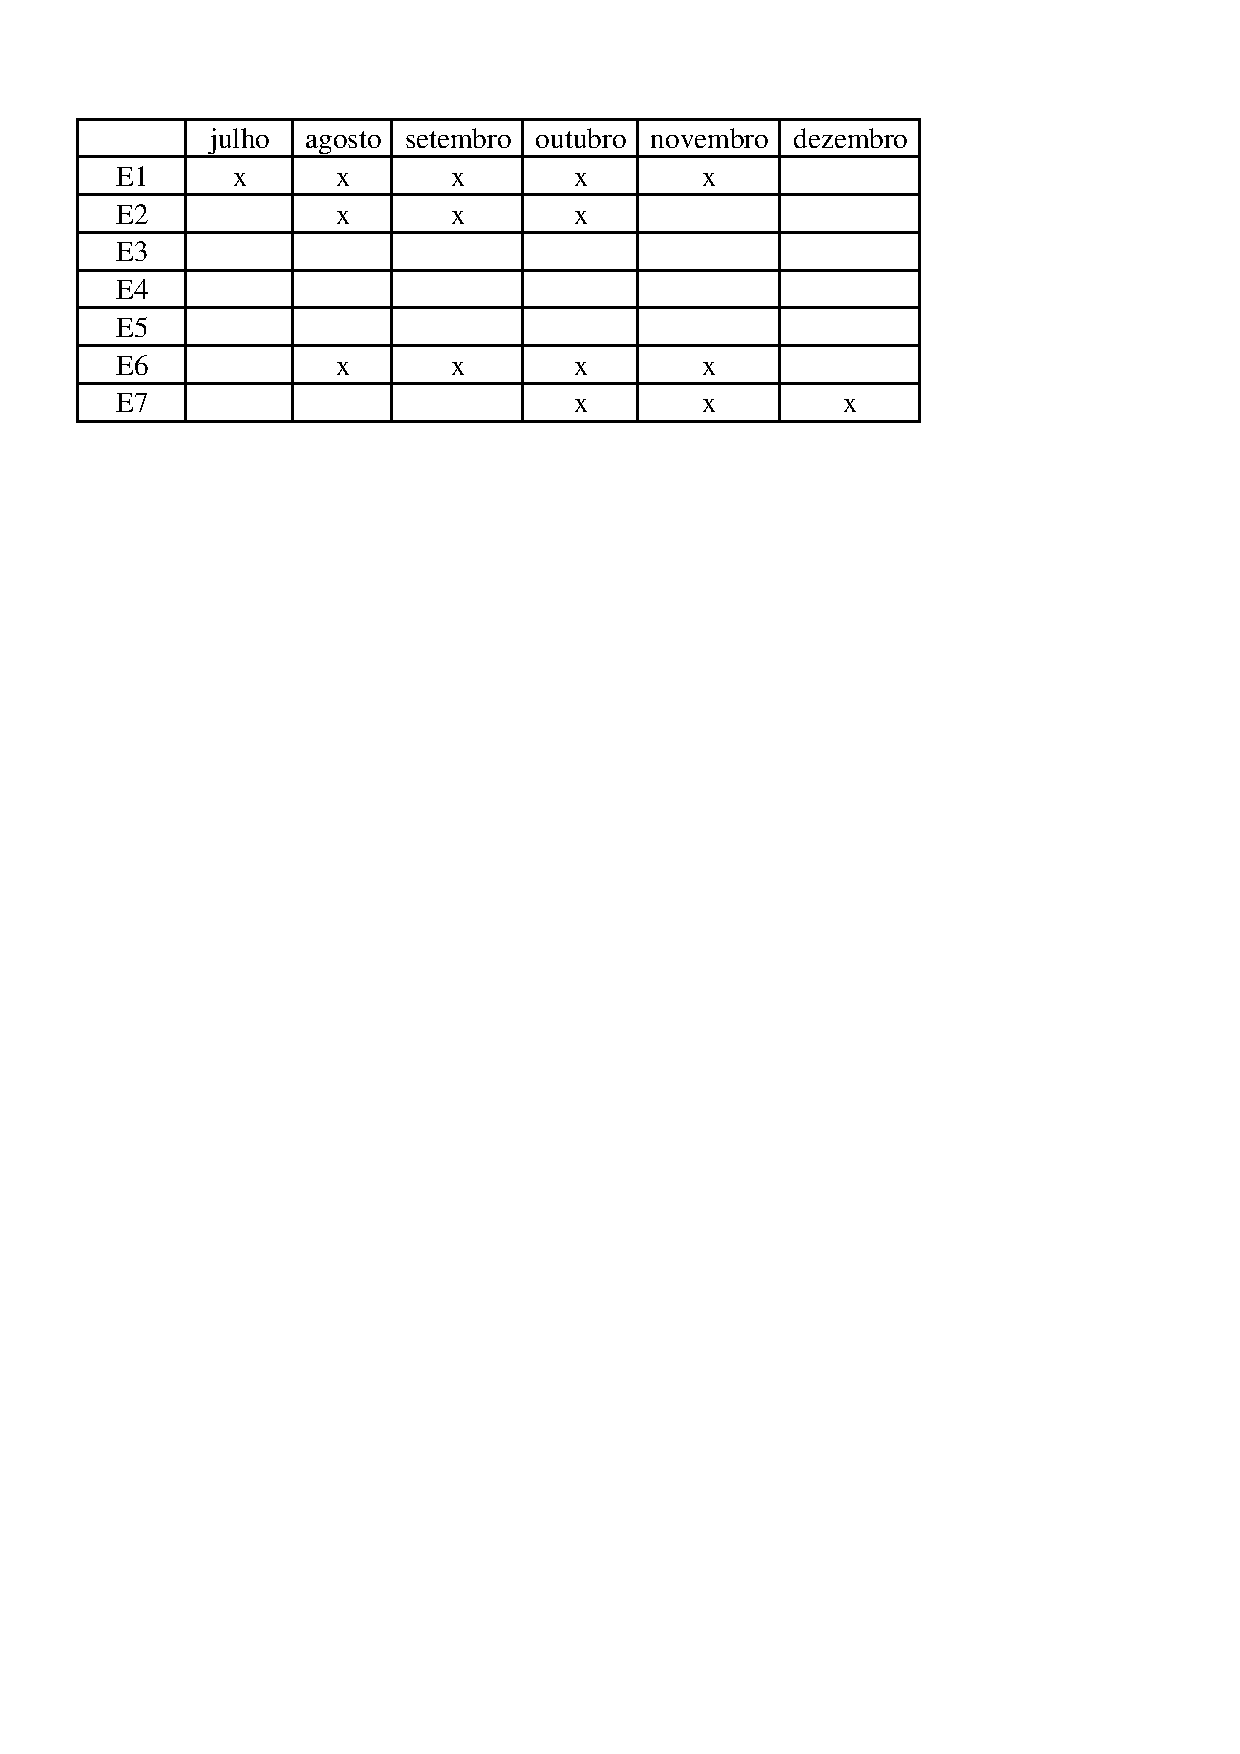
\includegraphics[clip, trim=1.3cm 22.5cm 5.4cm 2cm]{tudo/cronograma.pdf}
\end{table}



\chapter{Resultados parciais e esperados}

Neste capítulo serão apresentados os resultados parciais e esperados para o trabalho.

\section{Resultados parciais}

O modelo apresentado no \autoref{revisao_de_literatura}, apresentado por \cite{bragalli2012}, já se encontra adaptado a forma como a literatura brasileira, \citeonline{porto2006}, \citeonline{tsutiya2006}, \citeonline{neto1998}, \citeonline{nuvolari2003}, realiza o dimensionamento das redes de distribuição de água.

Testes iniciais com dados artificiais foram realizados e se mostraram promissores. Os valores obtidos com os testes do modelo foram iguais aos valores obtidos com algoritmos desenvolvidos em planilhas eletrônicas.


\section{Resultados esperados}

Obter um modelo testado, e confiável para dimensionar de forma otimizada redes de distribuição de água.
Melhorar o entendimento de como são dimensionadas as redes de distribuição de água, a formulação do dimensionamento como um problema de otimização combinatória tem esta virtude.
Espera-se disponibilizar uma ferramenta computacional para dar acessibilidade ao modelo proposto, e desta forma, facilitar que o publico em geral possa utilizar o modelo proposto no trabalho.




\citeonline{cormen2012} \citeonline{caliman2002}



%\citeonline{heller2006}
% https://books.google.com.br/books?hl=pt-BR&lr=&id=XFnnhzqetCoC&oi=fnd&pg=PA29&dq=hist%C3%B3ria+do+abastecimento+de+%C3%A1gua&ots=Hw9uoab_dk&sig=S7qD87qlSxLWDsOLYlMJbCTl4W4#v=onepage&q=hist%C3%B3ria%20do%20abastecimento%20de%20%C3%A1gua&f=false


% http://www.scielosp.org/pdf/rpsp/v25n6/v25n6a12.pdf

%\citeonline{tratabrasil}
% http://www.tratabrasil.org.br/por-que-a-universalizacao-do-saneamento-basico-e-uma-meta-tao-dificil-de-ser-atingida-no-brasil-pensar-brasil

%Pág 47

%	https://books.google.com.br/books?id=2kD9QBk16q4C&pg=PA43&lpg=PA43&dq=o+primeiro+sistema+de+aqueduto+na+Ass%C3%ADria+em+691+A.C&source=bl&ots=pLk1mUbHwd&sig=cQjH9R8x4765hEHgCm70w_2hHoo&hl=pt-BR&sa=X&ved=0ahUKEwjRx7X9wo7UAhXIhpAKHfBGAK0Q6AEINzAD#v=onepage&q=o%20primeiro%20sistema%20de%20aqueduto%20na%20Ass%C3%ADria%20em%20691%20A.C&f=false

%	http://www.tratabrasil.org.br/perdas-de-agua-desafios-ao-avanco-do-saneamento-basico-e-a-escassez-hidrica-2


%	http://www.brasil247.com/pt/247/amazonas247/174846/%C3%8Dndice-de-perda-de-%C3%A1gua-chega-a-755-em-Manaus.htm

%	http://www.scielo.br/scielo.php?script=sci_arttext&pid=S0101-74382010000100002

%	http://www.funasa.gov.br/site/wp-content/files_mf/reducao_de_perdas_em_saa74.pdf

%	http://revistadae.com.br/artigos/artigo_edicao_201_n_1622.pdf

%	https://scholar.google.com.br/scholar?hl=pt-BR&q=BAPTISTA%2C+M%C3%A1rcio+Benedito.+Hidr%C3%A1ulica+aplicada&btnG=&lr=

%	https://scholar.google.com.br/scholar?hl=pt-BR&q=BAPTISTA%2C+M%C3%A1rcio+Benedito.+Hidr%C3%A1ulica+aplicada&btnG=&lr=#



% Extras
% https://www.researchgate.net/profile/Harry_Schulz/publication/282813994_SIMULACAO_NUMERICA_DE_ESCOAMENTOS_SOBRE_AERADORES_FORMADOS_POR_ESCADA_E_CASCATA/links/561db25d08aef097132b2705.pdf
% https://www.researchgate.net/profile/Harry_Schulz/publication/259398891_FENOMENOS_DE_TRANSPORTE_E_HIDRAULICA_EXEMPLOS_DE_METODOS_NUMERICOS_E_COMPUTACIONAIS_PARA_A_RESOLUCAO_DE_PROBLEMAS/links/54d578950cf2970e4e64f52a.pdf

% http://www.deha.ufc.br/ticiana/Arquivos/Especializacao/Cariri/6_Sistemas%20de%20Abast%20de%20%C1gua/Manual%20UFC2.pdf



%http://anpur.org.br/app-urbana-2014/anais/html/gt4.html
% 
%Referência útil para a parte de Karina: http://www.rc.unesp.br/igce/aplicada/ead/estudos_ambientais/ea15.html


%%\newpage
%%
%%Este documento e seu código-fonte são exemplos de referência de uso da classe
%%\textsf{abntex2} e do pacote \textsf{abntex2cite}. O documento 
%%exemplifica a elaboração de trabalho acadêmico (tese, dissertação e outros do
%%gênero) produzido conforme a ABNT NBR 14724:2011 \emph{Informação e documentação
%%- Trabalhos acadêmicos - Apresentação}.
%%
%%
%%A expressão ``Modelo Canônico'' é utilizada para indicar que \abnTeX\ não é
%%modelo específico de nenhuma universidade ou instituição, mas que implementa tão
%%somente os requisitos das normas da ABNT. Uma lista completa das normas
%%observadas pelo \abnTeX\ é apresentada em \citeonline{abntex2classe}.
%%
%%Sinta-se convidado a participar do projeto \abnTeX! Acesse o site do projeto em
%%\url{http://www.abntex.net.br/}. Também fique livre para conhecer,
%%estudar, alterar e redistribuir o trabalho do \abnTeX, desde que os arquivos
%%modificados tenham seus nomes alterados e que os créditos sejam dados aos
%%autores originais, nos termos da ``The \LaTeX\ Project Public
%%License''\footnote{\url{http://www.latex-project.org/lppl.txt}}.
%%
%%Encorajamos que sejam realizadas customizações específicas deste exemplo para
%%universidades e outras instituições --- como capas, folha de aprovação, etc.
%%Porém, recomendamos que ao invés de se alterar diretamente os arquivos do
%%\abnTeX, distribua-se arquivos com as respectivas customizações.
%%Isso permite que futuras versões do \abnTeX~não se tornem automaticamente
%%incompatíveis com as customizações promovidas. Consulte
%%\citeonline{abntex2-wiki-como-customizar} par mais informações.
%%
%%Este documento deve ser utilizado como complemento dos manuais do \abnTeX\ 
%%\cite{abntex2classe,abntex2cite,abntex2cite-alf} e da classe \textsf{memoir}
%%\cite{memoir}. 
%%
%%Esperamos, sinceramente, que o \abnTeX\ aprimore a qualidade do trabalho que
%%você produzirá, de modo que o principal esforço seja concentrado no principal:
%%na contribuição científica.
%%
%%Equipe \abnTeX 
%%
%%Lauro César Araujo

% ----------------------------------------------------------
% PARTE
% ----------------------------------------------------------
%%\part{Preparação da pesquisa}
% ----------------------------------------------------------

% ---
% Capítulo com exemplos de comandos inseridos de arquivo externo 
% ---
%%%% abtex2-modelo-include-comandos.tex, v-1.9.6 laurocesar
%% Copyright 2012-2016 by abnTeX2 group at http://www.abntex.net.br/ 
%%
%% This work may be distributed and/or modified under the
%% conditions of the LaTeX Project Public License, either version 1.3
%% of this license or (at your option) any later version.
%% The latest version of this license is in
%%   http://www.latex-project.org/lppl.txt
%% and version 1.3 or later is part of all distributions of LaTeX
%% version 2005/12/01 or later.
%%
%% This work has the LPPL maintenance status `maintained'.
%% 
%% The Current Maintainer of this work is the abnTeX2 team, led
%% by Lauro César Araujo. Further information are available on 
%% http://www.abntex.net.br/
%%
%% This work consists of the files abntex2-modelo-include-comandos.tex
%% and abntex2-modelo-img-marca.pdf
%%

% ---
% Este capítulo, utilizado por diferentes exemplos do abnTeX2, ilustra o uso de
% comandos do abnTeX2 e de LaTeX.
% ---
 
\chapter{Resultados de comandos}\label{cap_exemplos}

\chapterprecis{Isto é uma sinopse de capítulo. A ABNT não traz nenhuma
normatização a respeito desse tipo de resumo, que é mais comum em romances 
e livros técnicos.}\index{sinopse de capítulo}

% ---
\section{Codificação dos arquivos: UTF8}
% ---

A codificação de todos os arquivos do \abnTeX\ é \texttt{UTF8}. É necessário que
você utilize a mesma codificação nos documentos que escrever, inclusive nos
arquivos de base bibliográficas |.bib|.

% ---
\section{Citações diretas}
\label{sec-citacao}
% ---

\index{citações!diretas}Utilize o ambiente \texttt{citacao} para incluir
citações diretas com mais de três linhas:

\begin{citacao}
As citações diretas, no texto, com mais de três linhas, devem ser
destacadas com recuo de 4 cm da margem esquerda, com letra menor que a do texto
utilizado e sem as aspas. No caso de documentos datilografados, deve-se
observar apenas o recuo \cite[5.3]{NBR10520:2002}.
\end{citacao}

Use o ambiente assim:

\begin{verbatim}
\begin{citacao}
As citações diretas, no texto, com mais de três linhas [...] deve-se observar
apenas o recuo \cite[5.3]{NBR10520:2002}.
\end{citacao}
\end{verbatim}

O ambiente \texttt{citacao} pode receber como parâmetro opcional um nome de
idioma previamente carregado nas opções da classe (\autoref{sec-hifenizacao}). Nesse
caso, o texto da citação é automaticamente escrito em itálico e a hifenização é
ajustada para o idioma selecionado na opção do ambiente. Por exemplo:

\begin{verbatim}
\begin{citacao}[english]
Text in English language in italic with correct hyphenation.
\end{citacao}
\end{verbatim}

Tem como resultado:

\begin{citacao}[english]
Text in English language in italic with correct hyphenation.
\end{citacao}

\index{citações!simples}Citações simples, com até três linhas, devem ser
incluídas com aspas. Observe que em \LaTeX as aspas iniciais são diferentes das
finais: ``Amor é fogo que arde sem se ver''.

% ---
\section{Notas de rodapé}
% ---

As notas de rodapé são detalhadas pela NBR 14724:2011 na seção 5.2.1\footnote{As
notas devem ser digitadas ou datilografadas dentro das margens, ficando
separadas do texto por um espaço simples de entre as linhas e por filete de 5
cm, a partir da margem esquerda. Devem ser alinhadas, a partir da segunda linha
da mesma nota, abaixo da primeira letra da primeira palavra, de forma a destacar
o expoente, sem espaço entre elas e com fonte menor
\citeonline[5.2.1]{NBR14724:2011}.}\footnote{Caso uma série de notas sejam
criadas sequencialmente, o \abnTeX\ instrui o \LaTeX\ para que uma vírgula seja
colocada após cada número do expoente que indica a nota de rodapé no corpo do
texto.}\footnote{Verifique se os números do expoente possuem uma vírgula para
dividi-los no corpo do texto.}. 


% ---
\section{Tabelas}
% ---

\index{tabelas}A \autoref{tab-nivinv} é um exemplo de tabela construída em
\LaTeX.

\begin{table}[htb]
\ABNTEXfontereduzida
\caption[Níveis de investigação]{Níveis de investigação.}
\label{tab-nivinv}
\begin{tabular}{p{2.6cm}|p{6.0cm}|p{2.25cm}|p{3.40cm}}
  %\hline
   \textbf{Nível de Investigação} & \textbf{Insumos}  & \textbf{Sistemas de Investigação}  & \textbf{Produtos}  \\
    \hline
    Meta-nível & Filosofia\index{filosofia} da Ciência  & Epistemologia &
    Paradigma  \\
    \hline
    Nível do objeto & Paradigmas do metanível e evidências do nível inferior &
    Ciência  & Teorias e modelos \\
    \hline
    Nível inferior & Modelos e métodos do nível do objeto e problemas do nível inferior & Prática & Solução de problemas  \\
   % \hline
\end{tabular}
\legend{Fonte: \citeonline{van86}}
\end{table}

Já a \autoref{tabela-ibge} apresenta uma tabela criada conforme o padrão do
\citeonline{ibge1993} requerido pelas normas da ABNT para documentos técnicos e
acadêmicos.

\begin{table}[htb]
\IBGEtab{%
  \caption{Um Exemplo de tabela alinhada que pode ser longa
  ou curta, conforme padrão IBGE.}%
  \label{tabela-ibge}
}{%
  \begin{tabular}{ccc}
  \toprule
   Nome & Nascimento & Documento \\
  \midrule \midrule
   Maria da Silva & 11/11/1111 & 111.111.111-11 \\
  \midrule 
   João Souza & 11/11/2111 & 211.111.111-11 \\
  \midrule 
   Laura Vicuña & 05/04/1891 & 3111.111.111-11 \\
  \bottomrule
\end{tabular}%
}{%
  \fonte{Produzido pelos autores.}%
  \nota{Esta é uma nota, que diz que os dados são baseados na
  regressão linear.}%
  \nota[Anotações]{Uma anotação adicional, que pode ser seguida de várias
  outras.}%
  }
\end{table}


% ---
\section{Figuras}
% ---

\index{figuras}Figuras podem ser criadas diretamente em \LaTeX,
como o exemplo da \autoref{fig_circulo}.

\begin{figure}[htb]
	\caption{\label{fig_circulo}A delimitação do espaço}
	\begin{center}
	    \setlength{\unitlength}{5cm}
		\begin{picture}(1,1)
		\put(0,0){\line(0,1){1}}
		\put(0,0){\line(1,0){1}}
		\put(0,0){\line(1,1){1}}
		\put(0,0){\line(1,2){.5}}
		\put(0,0){\line(1,3){.3333}}
		\put(0,0){\line(1,4){.25}}
		\put(0,0){\line(1,5){.2}}
		\put(0,0){\line(1,6){.1667}}
		\put(0,0){\line(2,1){1}}
		\put(0,0){\line(2,3){.6667}}
		\put(0,0){\line(2,5){.4}}
		\put(0,0){\line(3,1){1}}
		\put(0,0){\line(3,2){1}}
		\put(0,0){\line(3,4){.75}}
		\put(0,0){\line(3,5){.6}}
		\put(0,0){\line(4,1){1}}
		\put(0,0){\line(4,3){1}}
		\put(0,0){\line(4,5){.8}}
		\put(0,0){\line(5,1){1}}
		\put(0,0){\line(5,2){1}}
		\put(0,0){\line(5,3){1}}
		\put(0,0){\line(5,4){1}}
		\put(0,0){\line(5,6){.8333}}
		\put(0,0){\line(6,1){1}}
		\put(0,0){\line(6,5){1}}
		\end{picture}
	\end{center}
	\legend{Fonte: os autores}
\end{figure}

Ou então figuras podem ser incorporadas de arquivos externos, como é o caso da
\autoref{fig_grafico}. Se a figura que ser incluída se tratar de um diagrama, um
gráfico ou uma ilustração que você mesmo produza, priorize o uso de imagens
vetoriais no formato PDF. Com isso, o tamanho do arquivo final do trabalho será
menor, e as imagens terão uma apresentação melhor, principalmente quando
impressas, uma vez que imagens vetorias são perfeitamente escaláveis para
qualquer dimensão. Nesse caso, se for utilizar o Microsoft Excel para produzir
gráficos, ou o Microsoft Word para produzir ilustrações, exporte-os como PDF e
os incorpore ao documento conforme o exemplo abaixo. No entanto, para manter a
coerência no uso de software livre (já que você está usando \LaTeX e \abnTeX),
teste a ferramenta \textsf{InkScape}\index{InkScape}
(\url{http://inkscape.org/}). Ela é uma excelente opção de código-livre para
produzir ilustrações vetoriais, similar ao CorelDraw\index{CorelDraw} ou ao Adobe
Illustrator\index{Adobe Illustrator}. De todo modo, caso não seja possível
utilizar arquivos de imagens como PDF, utilize qualquer outro formato, como
JPEG, GIF, BMP, etc. Nesse caso, você pode tentar aprimorar as imagens
incorporadas com o software livre \textsf{Gimp}\index{Gimp}
(\url{http://www.gimp.org/}). Ele é uma alternativa livre ao Adobe
Photoshop\index{Adobe Photoshop}.

\begin{figure}[htb]
	\caption{\label{fig_grafico}Gráfico produzido em Excel e salvo como PDF}
	\begin{center}
	    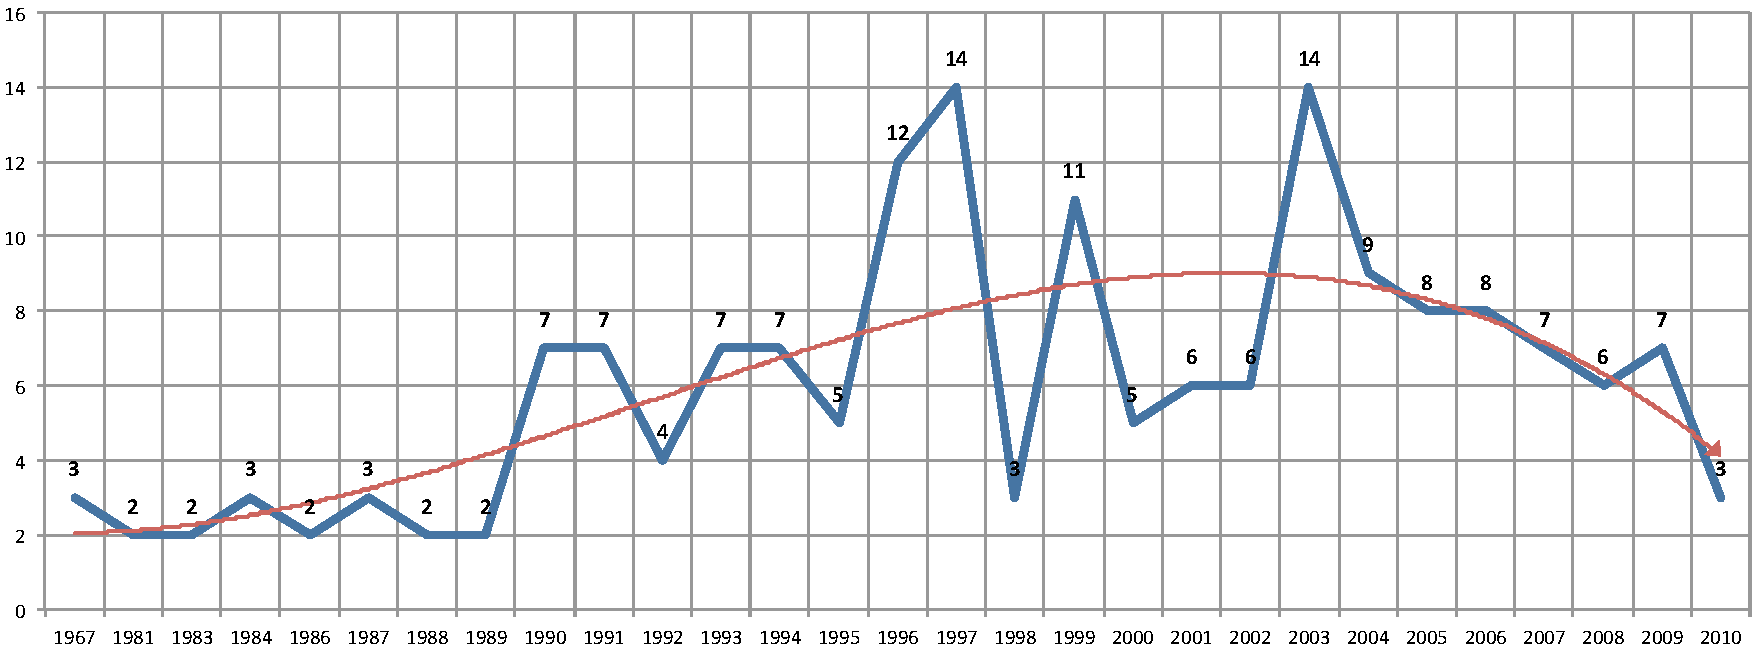
\includegraphics[scale=0.5]{abntex2-modelo-img-grafico.pdf}
	\end{center}
	\legend{Fonte: \citeonline[p. 24]{araujo2012}}
\end{figure}

% ---
\subsection{Figuras em \emph{minipages}}
% ---

\emph{Minipages} são usadas para inserir textos ou outros elementos em quadros
com tamanhos e posições controladas. Veja o exemplo da
\autoref{fig_minipage_imagem1} e da \autoref{fig_minipage_grafico2}.

\begin{figure}[htb]
 \label{teste}
 \centering
  \begin{minipage}{0.4\textwidth}
    \centering
    \caption{Imagem 1 da minipage} \label{fig_minipage_imagem1}
    
\includegraphics[scale=0.9]{abntex2-modelo-img-marca.pdf}
    \legend{Fonte: Produzido pelos autores}
  \end{minipage}
  \hfill
  \begin{minipage}{0.4\textwidth}
    \centering
    \caption{Grafico 2 da minipage} \label{fig_minipage_grafico2}
    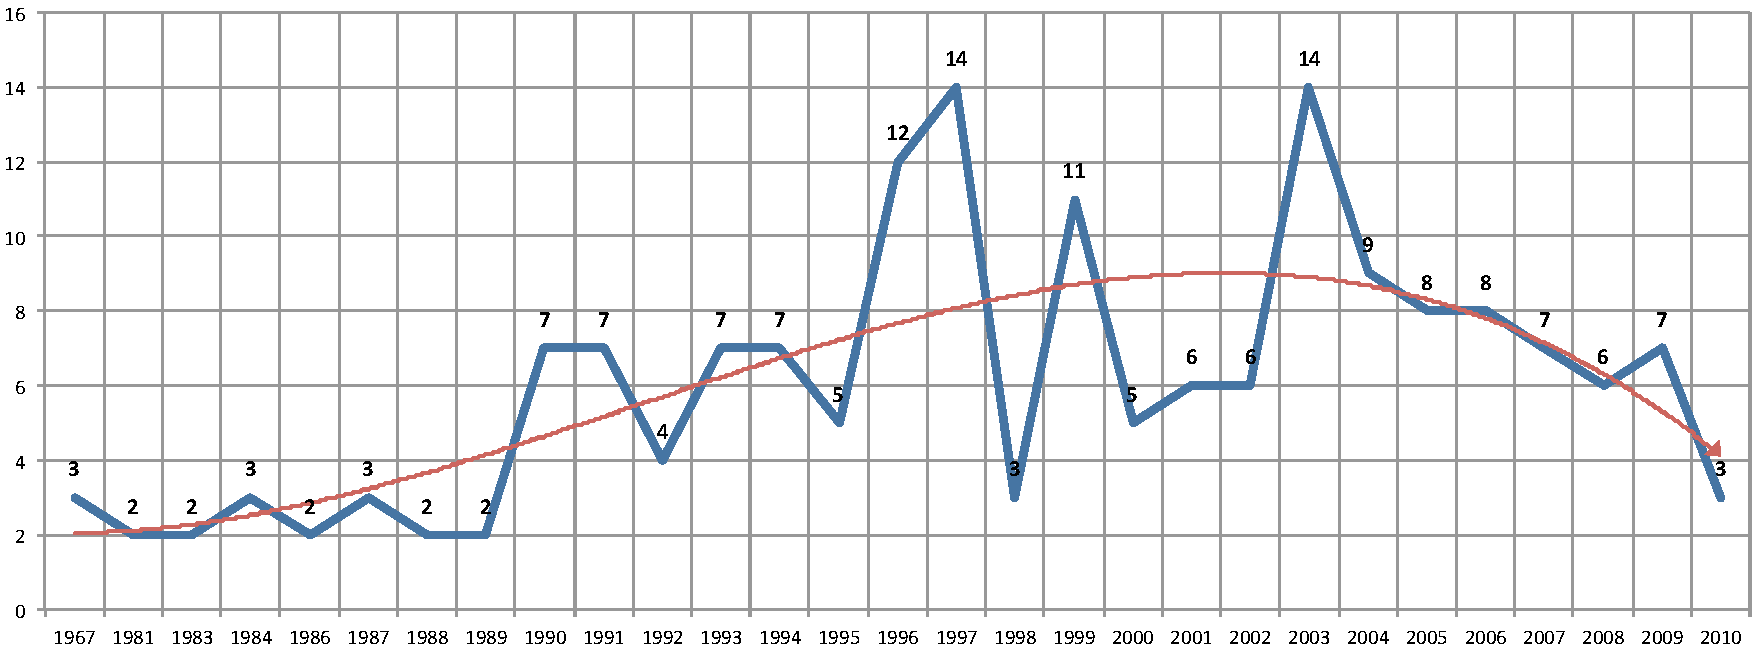
\includegraphics[scale=0.2]{abntex2-modelo-img-grafico.pdf}
    \legend{Fonte: \citeonline[p. 24]{araujo2012}}
  \end{minipage}
\end{figure}

Observe que, segundo a \citeonline[seções 4.2.1.10 e 5.8]{NBR14724:2011}, as
ilustrações devem sempre ter numeração contínua e única em todo o documento:

\begin{citacao}
Qualquer que seja o tipo de ilustração, sua identificação aparece na parte
superior, precedida da palavra designativa (desenho, esquema, fluxograma,
fotografia, gráfico, mapa, organograma, planta, quadro, retrato, figura,
imagem, entre outros), seguida de seu número de ordem de ocorrência no texto,
em algarismos arábicos, travessão e do respectivo título. Após a ilustração, na
parte inferior, indicar a fonte consultada (elemento obrigatório, mesmo que
seja produção do próprio autor), legenda, notas e outras informações
necessárias à sua compreensão (se houver). A ilustração deve ser citada no
texto e inserida o mais próximo possível do trecho a que se
refere. \cite[seções 5.8]{NBR14724:2011}
\end{citacao}

% ---
\section{Expressões matemáticas}
% ---

\index{expressões matemáticas}Use o ambiente \texttt{equation} para escrever
expressões matemáticas numeradas:

\begin{equation}
  \forall x \in X, \quad \exists \: y \leq \epsilon
\end{equation}

Escreva expressões matemáticas entre \$ e \$, como em $ \lim_{x \to \infty}
\exp(-x) = 0 $, para que fiquem na mesma linha.

Também é possível usar colchetes para indicar o início de uma expressão
matemática que não é numerada.

\[
\left|\sum_{i=1}^n a_ib_i\right|
\le
\left(\sum_{i=1}^n a_i^2\right)^{1/2}
\left(\sum_{i=1}^n b_i^2\right)^{1/2}
\]

Consulte mais informações sobre expressões matemáticas em
\url{https://github.com/abntex/abntex2/wiki/Referencias}.

% ---
\section{Enumerações: alíneas e subalíneas}
% ---

\index{alíneas}\index{subalíneas}\index{incisos}Quando for necessário enumerar
os diversos assuntos de uma seção que não possua título, esta deve ser
subdividida em alíneas \cite[4.2]{NBR6024:2012}:

\begin{alineas}

  \item os diversos assuntos que não possuam título próprio, dentro de uma mesma
  seção, devem ser subdivididos em alíneas; 
  
  \item o texto que antecede as alíneas termina em dois pontos;
  \item as alíneas devem ser indicadas alfabeticamente, em letra minúscula,
  seguida de parêntese. Utilizam-se letras dobradas, quando esgotadas as
  letras do alfabeto;

  \item as letras indicativas das alíneas devem apresentar recuo em relação à
  margem esquerda;

  \item o texto da alínea deve começar por letra minúscula e terminar em
  ponto-e-vírgula, exceto a última alínea que termina em ponto final;

  \item o texto da alínea deve terminar em dois pontos, se houver subalínea;

  \item a segunda e as seguintes linhas do texto da alínea começa sob a
  primeira letra do texto da própria alínea;
  
  \item subalíneas \cite[4.3]{NBR6024:2012} devem ser conforme as alíneas a
  seguir:

  \begin{alineas}
     \item as subalíneas devem começar por travessão seguido de espaço;

     \item as subalíneas devem apresentar recuo em relação à alínea;

     \item o texto da subalínea deve começar por letra minúscula e terminar em
     ponto-e-vírgula. A última subalínea deve terminar em ponto final, se não
     houver alínea subsequente;

     \item a segunda e as seguintes linhas do texto da subalínea começam sob a
     primeira letra do texto da própria subalínea.
  \end{alineas}
  
  \item no \abnTeX\ estão disponíveis os ambientes \texttt{incisos} e
  \texttt{subalineas}, que em suma são o mesmo que se criar outro nível de
  \texttt{alineas}, como nos exemplos à seguir:
  
  \begin{incisos}
    \item \textit{Um novo inciso em itálico};
  \end{incisos}
  
  \item Alínea em \textbf{negrito}:
  
  \begin{subalineas}
    \item \textit{Uma subalínea em itálico};
    \item \underline{\textit{Uma subalínea em itálico e sublinhado}}; 
  \end{subalineas}
  
  \item Última alínea com \emph{ênfase}.
  
\end{alineas}

% ---
\section{Espaçamento entre parágrafos e linhas}
% ---

\index{espaçamento!dos parágrafos}O tamanho do parágrafo, espaço entre a margem
e o início da frase do parágrafo, é definido por:

\begin{verbatim}
   \setlength{\parindent}{1.3cm}
\end{verbatim}

\index{espaçamento!do primeiro parágrafo}Por padrão, não há espaçamento no
primeiro parágrafo de cada início de divisão do documento
(\autoref{sec-divisoes}). Porém, você pode definir que o primeiro parágrafo
também seja indentado, como é o caso deste documento. Para isso, apenas inclua o
pacote \textsf{indentfirst} no preâmbulo do documento:

\begin{verbatim}
   \usepackage{indentfirst}      % Indenta o primeiro parágrafo de cada seção.
\end{verbatim}

\index{espaçamento!entre os parágrafos}O espaçamento entre um parágrafo e outro
pode ser controlado por meio do comando:

\begin{verbatim}
  \setlength{\parskip}{0.2cm}  % tente também \onelineskip
\end{verbatim}

\index{espaçamento!entre as linhas}O controle do espaçamento entre linhas é
definido por:

\begin{verbatim}
  \OnehalfSpacing       % espaçamento um e meio (padrão); 
  \DoubleSpacing        % espaçamento duplo
  \SingleSpacing        % espaçamento simples	
\end{verbatim}

Para isso, também estão disponíveis os ambientes:

\begin{verbatim}
  \begin{SingleSpace} ...\end{SingleSpace}
  \begin{Spacing}{hfactori} ... \end{Spacing}
  \begin{OnehalfSpace} ... \end{OnehalfSpace}
  \begin{OnehalfSpace*} ... \end{OnehalfSpace*}
  \begin{DoubleSpace} ... \end{DoubleSpace}
  \begin{DoubleSpace*} ... \end{DoubleSpace*} 
\end{verbatim}

Para mais informações, consulte \citeonline[p. 47-52 e 135]{memoir}.

% ---
\section{Inclusão de outros arquivos}\label{sec-include}
% ---

É uma boa prática dividir o seu documento em diversos arquivos, e não
apenas escrever tudo em um único. Esse recurso foi utilizado neste
documento. Para incluir diferentes arquivos em um arquivo principal,
de modo que cada arquivo incluído fique em uma página diferente, utilize o
comando:

\begin{verbatim}
   \include{documento-a-ser-incluido}      % sem a extensão .tex
\end{verbatim}

Para incluir documentos sem quebra de páginas, utilize:

\begin{verbatim}
   \input{documento-a-ser-incluido}      % sem a extensão .tex
\end{verbatim}

% ---
\section{Compilar o documento \LaTeX}
% ---

Geralmente os editores \LaTeX, como o
TeXlipse\footnote{\url{http://texlipse.sourceforge.net/}}, o
Texmaker\footnote{\url{http://www.xm1math.net/texmaker/}}, entre outros,
compilam os documentos automaticamente, de modo que você não precisa se
preocupar com isso.

No entanto, você pode compilar os documentos \LaTeX usando os seguintes
comandos, que devem ser digitados no \emph{Prompt de Comandos} do Windows ou no
\emph{Terminal} do Mac ou do Linux:

\begin{verbatim}
   pdflatex ARQUIVO_PRINCIPAL.tex
   bibtex ARQUIVO_PRINCIPAL.aux
   makeindex ARQUIVO_PRINCIPAL.idx 
   makeindex ARQUIVO_PRINCIPAL.nlo -s nomencl.ist -o ARQUIVO_PRINCIPAL.nls
   pdflatex ARQUIVO_PRINCIPAL.tex
   pdflatex ARQUIVO_PRINCIPAL.tex
\end{verbatim}

% ---
\section{Remissões internas}
% ---

Ao nomear a \autoref{tab-nivinv} e a \autoref{fig_circulo}, apresentamos um
exemplo de remissão interna, que também pode ser feita quando indicamos o
\autoref{cap_exemplos}, que tem o nome \emph{\nameref{cap_exemplos}}. O número
do capítulo indicado é \ref{cap_exemplos}, que se inicia à
\autopageref{cap_exemplos}\footnote{O número da página de uma remissão pode ser
obtida também assim:
\pageref{cap_exemplos}.}.
Veja a \autoref{sec-divisoes} para outros exemplos de remissões internas entre
seções, subseções e subsubseções.

O código usado para produzir o texto desta seção é:

\begin{verbatim}
Ao nomear a \autoref{tab-nivinv} e a \autoref{fig_circulo}, apresentamos um
exemplo de remissão interna, que também pode ser feita quando indicamos o
\autoref{cap_exemplos}, que tem o nome \emph{\nameref{cap_exemplos}}. O número
do capítulo indicado é \ref{cap_exemplos}, que se inicia à
\autopageref{cap_exemplos}\footnote{O número da página de uma remissão pode ser
obtida também assim:
\pageref{cap_exemplos}.}.
Veja a \autoref{sec-divisoes} para outros exemplos de remissões internas entre
seções, subseções e subsubseções.
\end{verbatim}

% ---
\section{Divisões do documento: seção}\label{sec-divisoes}
% ---

Esta seção testa o uso de divisões de documentos. Esta é a
\autoref{sec-divisoes}. Veja a \autoref{sec-divisoes-subsection}.

\subsection{Divisões do documento: subseção}\label{sec-divisoes-subsection}

Isto é uma subseção. Veja a \autoref{sec-divisoes-subsubsection}, que é uma
\texttt{subsubsection} do \LaTeX, mas é impressa chamada de ``subseção'' porque
no Português não temos a palavra ``subsubseção''.

\subsubsection{Divisões do documento: subsubseção}
\label{sec-divisoes-subsubsection}

Isto é uma subsubseção.

\subsubsection{Divisões do documento: subsubseção}

Isto é outra subsubseção.

\subsection{Divisões do documento: subseção}\label{sec-exemplo-subsec}

Isto é uma subseção.

\subsubsection{Divisões do documento: subsubseção}

Isto é mais uma subsubseção da \autoref{sec-exemplo-subsec}.


\subsubsubsection{Esta é uma subseção de quinto
nível}\label{sec-exemplo-subsubsubsection}

Esta é uma seção de quinto nível. Ela é produzida com o seguinte comando:

\begin{verbatim}
\subsubsubsection{Esta é uma subseção de quinto
nível}\label{sec-exemplo-subsubsubsection}
\end{verbatim}

\subsubsubsection{Esta é outra subseção de quinto nível}\label{sec-exemplo-subsubsubsection-outro}

Esta é outra seção de quinto nível.


\paragraph{Este é um parágrafo numerado}\label{sec-exemplo-paragrafo}

Este é um exemplo de parágrafo nomeado. Ele é produzida com o comando de
parágrafo:

\begin{verbatim}
\paragraph{Este é um parágrafo nomeado}\label{sec-exemplo-paragrafo}
\end{verbatim}

A numeração entre parágrafos numeradaos e subsubsubseções são contínuas.

\paragraph{Esta é outro parágrafo numerado}\label{sec-exemplo-paragrafo-outro}

Esta é outro parágrafo nomeado.

% ---
\section{Este é um exemplo de nome de seção longo. Ele deve estar
alinhado à esquerda e a segunda e demais linhas devem iniciar logo abaixo da
primeira palavra da primeira linha}
% ---

Isso atende à norma \citeonline[seções de 5.2.2 a 5.2.4]{NBR14724:2011} 
 e \citeonline[seções de 3.1 a 3.8]{NBR6024:2012}.

% ---
\section{Diferentes idiomas e hifenizações}
\label{sec-hifenizacao}
% ---

Para usar hifenizações de diferentes idiomas, inclua nas opções do documento o
nome dos idiomas que o seu texto contém. Por exemplo (para melhor
visualização, as opções foram quebras em diferentes linhas):

\begin{verbatim}
\documentclass[
	12pt,
	openright,
	twoside,
	a4paper,
	english,
	french,
	spanish,
	brazil
	]{abntex2}
\end{verbatim}

O idioma português-brasileiro (\texttt{brazil}) é incluído automaticamente pela
classe \textsf{abntex2}. Porém, mesmo assim a opção \texttt{brazil} deve ser
informada como a última opção da classe para que todos os pacotes reconheçam o
idioma. Vale ressaltar que a última opção de idioma é a utilizada por padrão no
documento. Desse modo, caso deseje escrever um texto em inglês que tenha
citações em português e em francês, você deveria usar o preâmbulo como abaixo:

\begin{verbatim}
\documentclass[
	12pt,
	openright,
	twoside,
	a4paper,
	french,
	brazil,
	english
	]{abntex2}
\end{verbatim}

A lista completa de idiomas suportados, bem como outras opções de hifenização,
estão disponíveis em \citeonline[p.~5-6]{babel}.

Exemplo de hifenização em inglês\footnote{Extraído de:
\url{http://en.wikibooks.org/wiki/LaTeX/Internationalization}}:

\begin{otherlanguage*}{english}
\textit{Text in English language. This environment switches all language-related
definitions, like the language specific names for figures, tables etc. to the other
language. The starred version of this environment typesets the main text
according to the rules of the other language, but keeps the language specific
string for ancillary things like figures, in the main language of the document.
The environment hyphenrules switches only the hyphenation patterns used; it can
also be used to disallow hyphenation by using the language name
`nohyphenation'.}
\end{otherlanguage*}

Exemplo de hifenização em francês\footnote{Extraído de:
\url{http://bigbrowser.blog.lemonde.fr/2013/02/17/tu-ne-tweeteras-point-le-vatican-interdit-aux-cardinaux-de-tweeter-pendant-le-conclave/}}:

\begin{otherlanguage*}{french}
\textit{Texte en français. Pas question que Twitter ne vienne faire une
concurrence déloyale à la traditionnelle fumée blanche qui marque l'élection
d'un nouveau pape. Pour éviter toute fuite précoce, le Vatican a donc pris un
peu d'avance, et a déjà interdit aux cardinaux qui prendront part au vote
d'utiliser le réseau social, selon Catholic News Service. Une mesure valable
surtout pour les neuf cardinaux – sur les 117 du conclave – pratiquants très
actifs de Twitter, qui auront interdiction pendant toute la période de se
connecter à leur compte.}
\end{otherlanguage*}

Pequeno texto em espanhol\footnote{Extraído de:
\url{http://internacional.elpais.com/internacional/2013/02/17/actualidad/1361102009_913423.html}}:

\foreignlanguage{spanish}{\textit{Decenas de miles de personas ovacionan al pontífice en su
penúltimo ángelus dominical, el primero desde que anunciase su renuncia. El Papa se
centra en la crítica al materialismo}}.

O idioma geral do texto por ser alterado como no exemplo seguinte:

\begin{verbatim}
  \selectlanguage{english}
\end{verbatim}

Isso altera automaticamente a hifenização e todos os nomes constantes de
referências do documento para o idioma inglês. Consulte o manual da classe
\cite{abntex2classe} para obter orientações adicionais sobre internacionalização de
documentos produzidos com \abnTeX.

A \autoref{sec-citacao} descreve o ambiente \texttt{citacao} que pode receber
como parâmetro um idioma a ser usado na citação.

% ---
\section{Consulte o manual da classe \textsf{abntex2}}
% ---

Consulte o manual da classe \textsf{abntex2} \cite{abntex2classe} para uma
referência completa das macros e ambientes disponíveis. 

Além disso, o manual possui informações adicionais sobre as normas ABNT
observadas pelo \abnTeX\ e considerações sobre eventuais requisitos específicos
não atendidos, como o caso da \citeonline[seção 5.2.2]{NBR14724:2011}, que
especifica o espaçamento entre os capítulos e o início do texto, regra
propositalmente não atendida pelo presente modelo.

% ---
\section{Referências bibliográficas}
% ---

A formatação das referências bibliográficas conforme as regras da ABNT são um
dos principais objetivos do \abnTeX. Consulte os manuais
\citeonline{abntex2cite} e \citeonline{abntex2cite-alf} para obter informações
sobre como utilizar as referências bibliográficas.

%-
\subsection{Acentuação de referências bibliográficas}
%-

Normalmente não há problemas em usar caracteres acentuados em arquivos
bibliográficos (\texttt{*.bib}). Porém, como as regras da ABNT fazem uso quase
abusivo da conversão para letras maiúsculas, é preciso observar o modo como se
escreve os nomes dos autores. Na ~\autoref{tabela-acentos} você encontra alguns
exemplos das conversões mais importantes. Preste atenção especial para `ç' e `í'
que devem estar envoltos em chaves. A regra geral é sempre usar a acentuação
neste modo quando houver conversão para letras maiúsculas.

\begin{table}[htbp]
\caption{Tabela de conversão de acentuação.}
\label{tabela-acentos}

\begin{center}
\begin{tabular}{ll}\hline\hline
acento & \textsf{bibtex}\\
à á ã & \verb+\`a+ \verb+\'a+ \verb+\~a+\\
í & \verb+{\'\i}+\\
ç & \verb+{\c c}+\\
\hline\hline
\end{tabular}
\end{center}
\end{table}


% ---
\section{Precisa de ajuda?}
% ---

Consulte a FAQ com perguntas frequentes e comuns no portal do \abnTeX:
\url{https://github.com/abntex/abntex2/wiki/FAQ}.

Inscreva-se no grupo de usuários \LaTeX:
\url{http://groups.google.com/group/latex-br}, tire suas dúvidas e ajude
outros usuários.

Participe também do grupo de desenvolvedores do \abnTeX:
\url{http://groups.google.com/group/abntex2} e faça sua contribuição à
ferramenta.

% ---
\section{Você pode ajudar?}
% ---

Sua contribuição é muito importante! Você pode ajudar na divulgação, no
desenvolvimento e de várias outras formas. Veja como contribuir com o \abnTeX\
em \url{https://github.com/abntex/abntex2/wiki/Como-Contribuir}.

% ---
\section{Quer customizar os modelos do \abnTeX\ para sua instituição ou
universidade?}
% ---

Veja como customizar o \abnTeX\ em:
\url{https://github.com/abntex/abntex2/wiki/ComoCustomizar}.


% ---

% ----------------------------------------------------------
% PARTE
% ----------------------------------------------------------
%%\part{Referenciais teóricos}
% ----------------------------------------------------------

% ---
% Capítulo de revisão de literatura
% ---
%%\chapter{Lorem ipsum dolor sit amet}
% ---

% ---
%%\section{Aliquam vestibulum fringilla lorem}
% ---

%%\lipsum[1]

%%\lipsum[2-3]

% ----------------------------------------------------------
% PARTE
% ----------------------------------------------------------
%%\part{Resultados}
% ----------------------------------------------------------

% ---
% primeiro capítulo de Resultados
% ---
%%\chapter{Lectus lobortis condimentum}
% ---

% ---
%%\section{Vestibulum ante ipsum primis in faucibus orci luctus et ultrices
%%posuere cubilia Curae}
% ---

%%\lipsum[21-22]

% ---
% segundo capítulo de Resultados
% ---
%%\chapter{Nam sed tellus sit amet lectus urna ullamcorper tristique interdum elementum}
% ---

% ---
%%\section{Pellentesque sit amet pede ac sem eleifend consectetuer}
% ---

%%\lipsum[24]

% ----------------------------------------------------------
% Finaliza a parte no bookmark do PDF
% para que se inicie o bookmark na raiz
% e adiciona espaço de parte no Sumário
% ----------------------------------------------------------
\phantompart

% ---
% Conclusão
% ---
%%\chapter{Conclusão}
% ---

%%\lipsum[31-33]

% ----------------------------------------------------------
% ELEMENTOS PÓS-TEXTUAIS
% ----------------------------------------------------------
\postextual
% ----------------------------------------------------------

% ----------------------------------------------------------
% Referências bibliográficas
% ----------------------------------------------------------
\bibliography{abntex2-modelo-references}

% ----------------------------------------------------------
% Glossário
% ----------------------------------------------------------
%
% Consulte o manual da classe abntex2 para orientações sobre o glossário.
%
%\glossary

% ----------------------------------------------------------
% Apêndices
% ----------------------------------------------------------

% ---
% Inicia os apêndices
% ---
%%\begin{apendicesenv}

% Imprime uma página indicando o início dos apêndices
%%\partapendices

% ----------------------------------------------------------
%%\chapter{Quisque libero justo}
% ----------------------------------------------------------

%%\lipsum[50]

% ----------------------------------------------------------
%%\chapter{Nullam elementum urna vel imperdiet sodales elit ipsum pharetra ligula
%%ac pretium ante justo a nulla curabitur tristique arcu eu metus}
% ----------------------------------------------------------
%%\lipsum[55-57]

%%\end{apendicesenv}
% ---


% ----------------------------------------------------------
% Anexos
% ----------------------------------------------------------

% ---
% Inicia os anexos
% ---
%%\begin{anexosenv}

% Imprime uma página indicando o início dos anexos
%%\partanexos

% ---
%%\chapter{Morbi ultrices rutrum lorem.}
% ---
%%\lipsum[30]

% ---
%%\chapter{Cras non urna sed feugiat cum sociis natoque penatibus et magnis dis
%%parturient montes nascetur ridiculus mus}
% ---

%%\lipsum[31]

% ---
%%\chapter{Fusce facilisis lacinia dui}
% ---

%%\lipsum[32]

%%\end{anexosenv}

%---------------------------------------------------------------------
% INDICE REMISSIVO
%---------------------------------------------------------------------
\phantompart
\printindex
%---------------------------------------------------------------------

\end{document}



%Conjuntos do modelo \\
%\noindent
%$\setN$ = conjunto de nos. \\
%$\setE$ = conjunto de canos. \\
%$\setS$ = conjunto de fontes (reservatórios). \\
%$\delta_{+}$ = conjunto de canos saindo do nó $\mathrm{i}$ $\left( \mathrm{i} \in \mathbb{N} \right)$. \\
%$\delta_{-}$ = conjunto de canos entrando do nó $\mathrm{i}$ $\left( \mathrm{i} \in \mathbb{N} \right)$. \\
%$\setT$ = conjunto das vazões máximas para um diâmetro. \\
%
%Parâmetros do modelo \\
%\noindent
%$\ell \!\left( \edge \right)$ = comprimento do cano $\edge$ $\left( \edge \in \setE \right)$, em m. \\ 
%$\dmin \!\left( \edge \right)$ = diâmetro mínimo do cano $\edge$ $\left( \edge \in \setE \right)$, em m. \\
%$\dmax \!\left( \edge \right)$ = diâmetro máximo do cano $\edge$ $\left( \edge \in \setE \right)$, em m. \\
%$\dem\!\left( \inode \right)$ = demanda no nó $\inode$ $\left( \inode \in \setN \right)$, em $\mathrm{m^{3}/s}$. \\
%$\z\!\left( \inode \right)$ = cota do nó $\inode$ $\left( \inode \in \setN \cup \setS \right)$, em m. \\
%$\phmin\!\left( \inode \right)$ = pressão mínima no nó $\inode$ $\left( \inode \in \setN \right)$, em m. \\
%$\dmin := \DT\left( \edge, 1 \right) < \DT\left( \edge, 2 \right) < \cdots < \DT\left( \edge, \mathrm{r_{e}} \right) := \dmax$  \\
%$\C$ = constante da rugosidade dos canos, adimensional. \\
%$\q$ = taxa de contribuição linear $\mathrm{m^{3}/(Km \cdot s)}$. \\
%
%
%Variáveis do modelo \\
%\noindent
%$\vQ \!\left( \edge \right)$ = vazão no cano $\edge$ $\left(\forall \edge \in \setE \right)$, em $\mathrm{m^{3}/s}$. \\
%$\vQF \!\left( \edge \right)$ = vazão média no cano $\edge$ $\left(\forall \edge \in \setE \right)$, em $\mathrm{m^{3}/s}$. \\
%$\vD \!\left( \edge \right)$ = diâmetro do cano $\edge$ $\left(\forall \edge \in \setE \right)$, em m. \\
%$\vH \!\left( \inode \right)$ = pressão no nó $\inode$ $\left(\forall \inode \in \setN \right)$, em m. \\
%
%
%Restrições do modelo \\
%\noindent
%\begin{equation} 
%	\dmin \leq \vD\!\left( \edge \right) \leq \dmax \left(\forall \edge \in \setE \right)
%\end{equation}
%
%\begin{equation} 
%	\phmin + \z\!\left( \inode \right) \leq \vH \!\left( \inode \right) \left(\forall \inode \in \setN \right)
%\end{equation}
%
%
%\begin{equation} 
%	\phmin + \z\!\left( \inode' \right) = \vH \!\left( \inode' \right) \left(\exists! \ \inode' \in \setN \right)
%\end{equation}
%
%\begin{equation} 
%	\vQ\!\left( \edge \right)\leq \tilde{\mathrm{Q}}\!\left( \tT \right) \left( \forall \edge \in \setE , \ \exists \ \tT \in \setT \right)
%\end{equation}
%
%\begin{equation} 
%	\vQT\!\left( \edge \right) = \q\ell\!\left( \edge \right) \left(\forall \edge \in \setE \right)
%\end{equation}
%	
%\begin{equation} 
%	\vQF\!\left( \edge \right) = \dfrac{2\vQ\!\left( \edge \right) - \vQT\!\left( \edge \right)}{2} \left(\forall \edge \in \setE \right)
%\end{equation}
%
%
%Fluxo
%\begin{equation}
%\sum_{\edge \in \setdn\!\left( \inode \right)} \!\!\!\vQ \! \left( \edge \right) - \sum_{\edge \in 	\setdp\!\left( \inode \right)} \!\!\! \vQ \!\left( \edge \right) =  \dem\!\left( \inode \right), \left(\forall \inode \in \setN \right)
%\end{equation}
%
%
%Perda de pressão
%\begin{equation}
%\vH\!\left( \inode \right) - \vH\!\left( \jnode \right) = \dfrac{10.7 \ell \!\left( \edge \right)\vQF\!\left( \edge \right)^{1.852}}{\C\!\left( \edge \right)^{1.852}\vD\!\left( \edge \right)^{4.87}}, \left(\forall \edge = (\inode, \jnode) \in \setE \right)
%\end{equation}
%
%Objetivo
%\begin{equation}
%	\mathrm{minimize} \sum_{\edge} \vD\!\left( \edge \right), \left(\edge \in \setE \right)
%\end{equation}

